\section{ALU}
This section describes the ALU(arithmetic logic unit). Our implementation of the ALU has three parallel data buses consisting of two 32bit input operands and a 32bit result output. Furthermore, there is an 6bit input for the opcode. The ALU can perform 7 operations: add, sub, and, or, sll, slt and interconnect one of the two inputs to the result output. Additionally, there is an zero output flag if the operation results in zero.

\begin{figure}[h!]
  \centering
  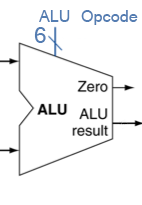
\includegraphics[width=0.8\textwidth]{figure/alu.png}
  \caption{ALU}
  \label{fig:ALU}
\end{figure}
